\documentclass[border=10pt]{standalone}

\usepackage{tikz}
\usepackage{tikzsymbols}
\usetikzlibrary{calc,patterns,shapes.geometric}

\def\centerarc[#1](#2)(#3:#4:#5){\draw[#1] ($(#2)+({#5*cos(#3)},{#5*sin(#3)})$) arc (#3:#4:#5);}

\begin{document}
	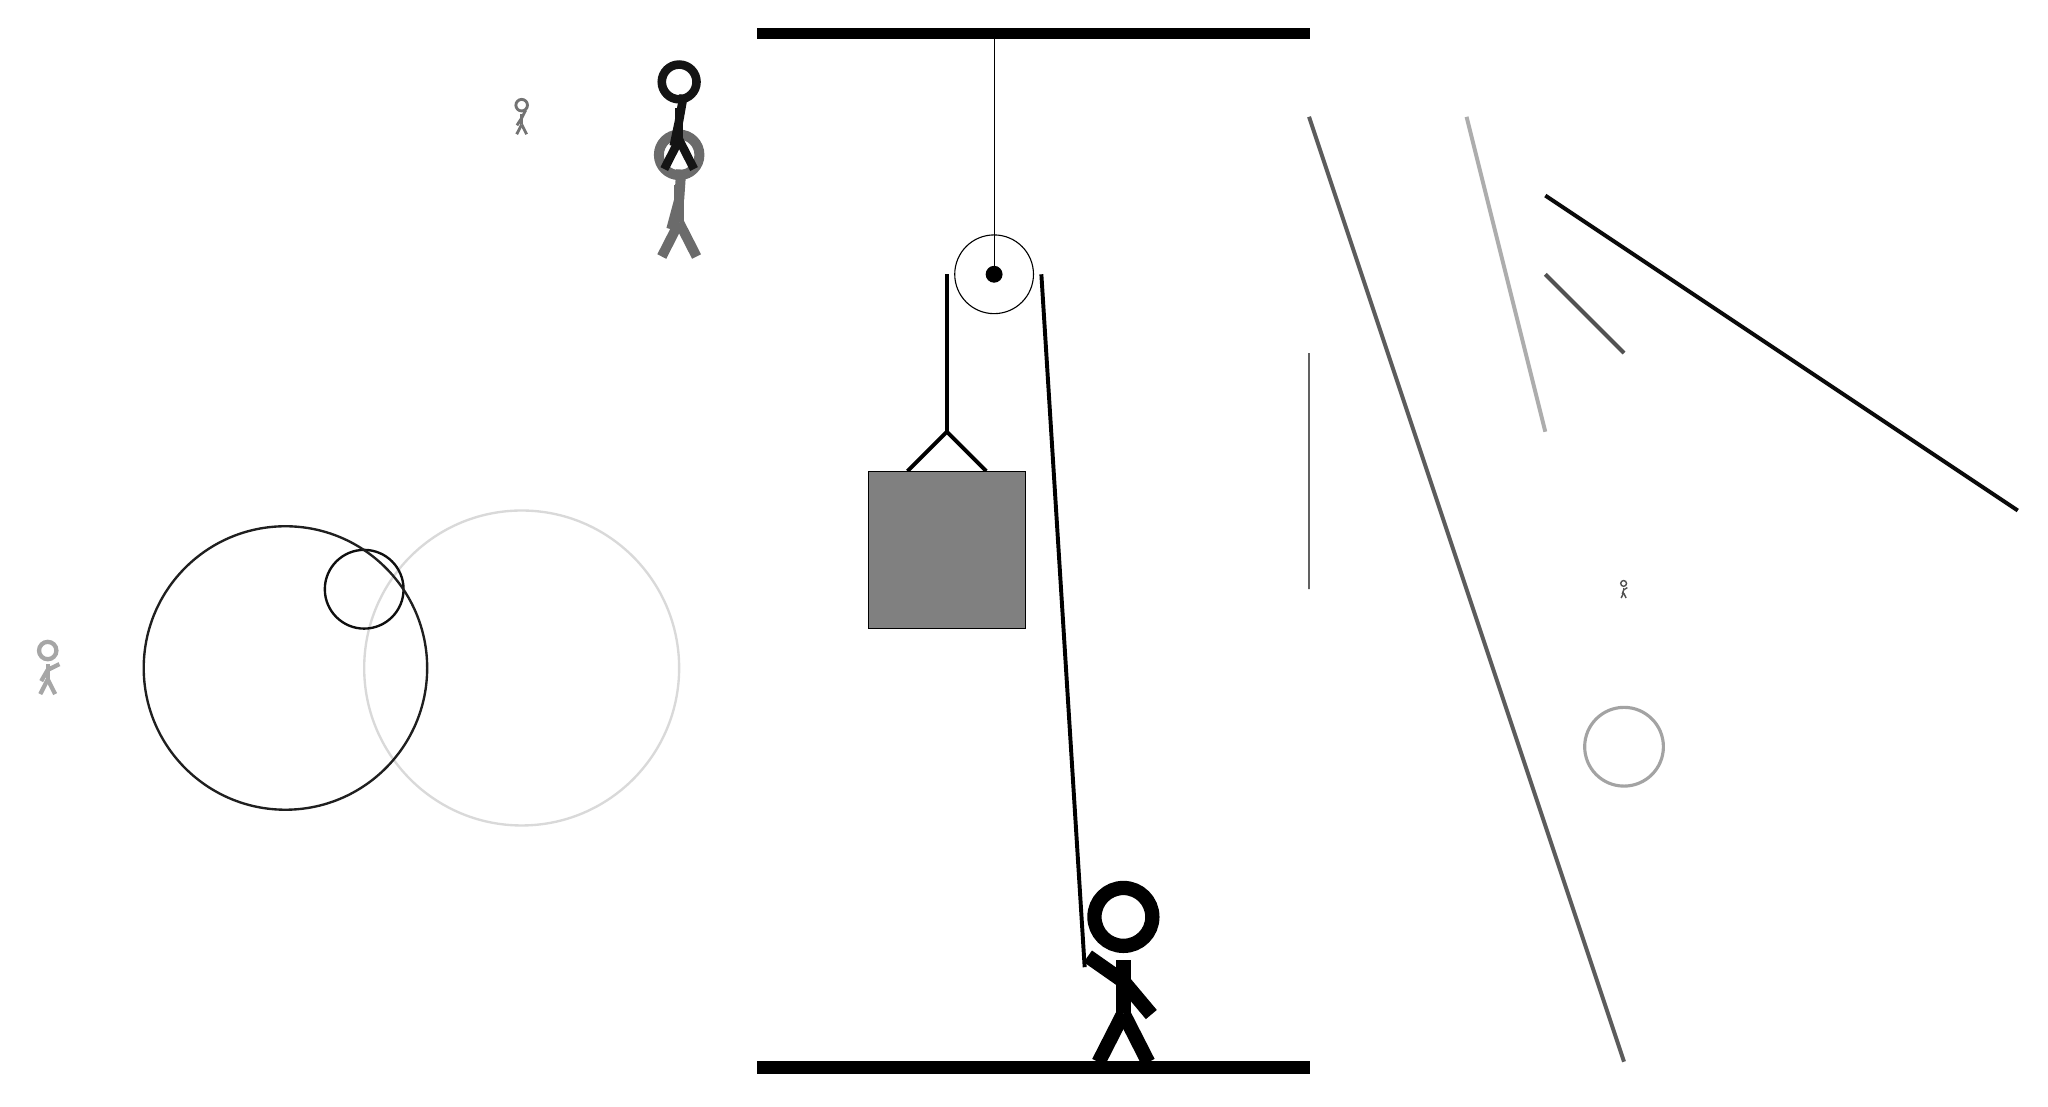
\begin{tikzpicture}
		%%%%% START %%%%%
		
		\draw[fill=black] (-2, 10) rectangle (5, 10.125);
		
		\draw[line width=0.5mm, color=black!64](9, -3) -- (5, 9);
		
		\node[line width=0.4mm, color=black!58] at (-3, 8) {\Strichmaxerl[7][75][86]};
		\draw [line width=0.3mm, color=black!15](-5, 2) circle (2.0);
		\draw[line width=0.5mm, color=black!68](8, 7) -- (9, 6);
		\node[line width=0.7mm, color=black!55] at (-5, 9) {\Strichmaxerl[2][57][63]};
		\draw[line width=0.5mm, color=black!96](8, 8) -- (14, 4);
		\draw[line width=0.5mm, color=black!32](8, 5) -- (7, 9);
		\node[line width=0.5mm, color=black!92] at (-3, 9) {\Strichmaxerl[6][78][80]};
		\draw [line width=0.3mm, color=black!94](-7, 3) circle (0.5);
		\node[line width=0.5mm, color=black!68] at (9, 3) {\Strichmaxerl[1][72][31]};
		\draw [line width=0.4mm, color=black!36](9, 1) circle (0.5);
		
		\draw [line width=0.3mm, color=black!88](-8, 2) circle (1.8);
		\node[line width=0.2mm, color=black!35] at (-11, 2) {\Strichmaxerl[3][60][26]};
		
		\draw[line width=0.3mm, color=black!62] (5, 6) rectangle (5, 3);
		
		\draw (1, 7) circle (0.5);
		\draw[fill=black] (1, 7) circle (0.1);
		\draw (1, 10) -- (1, 7);
		
		\draw[line width=0.5mm] (-0.1, 4.5) -- (0.4, 5.0) -- (0.9, 4.5);
		\draw[fill=black!50] (-0.6, 4.5) rectangle (1.4, 2.5);
		
		\draw[line width=0.5mm] (0.4, 7) -- (0.4, 5.0);
		\centerarc[line width=0.5mm](1, 7)(0:180:0.6);
		\draw[line width=0.5mm](1.6, 7) -- (2.15, -1.8);
		
		\node at (2.6, -1.9) {\Strichmaxerl[10][-35][-50]};
		
		\draw[fill=black] (-2, -3) rectangle (5, -3.15);
		
		%%%%% END %%%%%
	\end{tikzpicture}
\end{document}